\documentclass[conference]{IEEEtran}
\renewcommand\IEEEkeywordsname{keywords}
\usepackage{graphicx}
\usepackage{epstopdf}
\usepackage{float}
\usepackage{amssymb}
\usepackage{multirow}
\usepackage[english]{babel}
\usepackage{algorithmic,algorithm}
\renewcommand{\algorithmicrequire}{\textbf{Input:}}
\renewcommand{\algorithmicensure}{\textbf{Output:}}
\usepackage{enumerate}
\usepackage{lipsum}% http://ctan.org/pkg/lipsum
\hyphenation{op-tical net-works semi-conduc-tor}
\usepackage{booktabs}
\usepackage{amsmath}
\usepackage[smallscripts]{moresize}
%\usepackage[numbers,sort&compress]{natbib}
\usepackage[numbers,sort]{natbib}
\usepackage[most]{tcolorbox}
%\usepackage{ctable}

\begin{document}

\title{Introduction to Convolutional Neural Networks for Image-based Disease Detection in Tomato Plants}
%%%%%%%%%%%%%%%%%%%%%%%%%%%%%%%%%%%%%%%
% \author{\IEEEauthorblockN{Utpal Kant Singh, Rajnish Kumar, Saurabh Kumar, Shibasish Kar, Santos Kumar Baliarsingh}

% \IEEEauthorblockA{School of Computer Engineering,
% KIIT Deemed to be University, Bhubaneswar, 751024, India}
% \{20051117, 2005118, 20051096, 2005335, santos.baliarsinghfcs\}@kiit.ac.in
% }
%%%%%%%%%%%%%%%%%%%%%%%%%%%%%%%%%%%%
\author{\IEEEauthorblockN{Utpal Kant Singh}
\IEEEauthorblockA{School of Computer Engineering\\
KIIT Deemed to be University,\\ Bhubaneswar, India 751024\\
Email: utpalkant.4855@gmail.com}
\and
\IEEEauthorblockN{Vishal R. Satpute}
\IEEEauthorblockA{Department of Electronics and \\Communication Engineering\\
VNIT, Nagpur, India 440010\\
Email: vrsatpute@ece.vnit.ac.in}
}
%%%%%%%%%%%%%%%%%%%%%%%%%%%%%%%%%%%%%%%%%%%%%


\maketitle

\begin{abstract}

Tomatoes are extensively cultivated in India due to their adaptability to the country's tropical climate. However, various factors, including climate conditions, can hinder tomato growth and lead to reduced yield. Plant diseases pose a significant threat to agricultural productivity and can result in substantial financial losses. Traditional methods of disease detection for tomato crops have been ineffective and time-consuming. Early detection of diseases is crucial for better outcomes. To address this, the study explores the application of deep learning techniques, specifically convolutional neural networks (CNNs), for identifying tomato leaf diseases using computer vision technology. The research demonstrates the effectiveness of the proposed approach, achieving an average accuracy of 95\% in disease classification. This method shows promise in enabling early detection and timely management of tomato leaf diseases, thereby improving crop productivity and quality. \\

 
\end{abstract}


\begin{IEEEkeywords}
Convolutional Neural Network, Deep Learning, Machine Learning, Tomato Leaf Disease Detection, 
\end{IEEEkeywords}
 
\IEEEpeerreviewmaketitle



\section{Introduction}



\subsection{Motivation}
The Indian economy is heavily dependent on agriculture, with farmers growing a wide range of products, including tomatoes. Because tomato crops are prone to disease, there may be substantial yield and quality losses. For farmers to safeguard their means of subsistence, early diagnosis and treatment of these illnesses are essential. Pesticides are one example of a traditional disease management strategy that might have a harmful environmental impact. Early disease detection encourages sustainable agriculture practises by reducing the need for chemical treatments. Some tomato illnesses can endanger human health by contaminating produce or exposing people to toxins. These hazards can be reduced by early illness detection and treatment. Manual inspection-based conventional disease detection techniques are expensive and resource-intensive. Automated methods that are effective and trustworthy in spotting tomato illnesses are becoming more and more necessary. \\ 

In the fields of object identification and picture classification, convolutional neural networks (CNNs) have made tremendous strides. The way we recognise and control plant diseases may be completely altered by the use of CNNs to disease detection. Early disease identification is made possible by CNNs, enabling for prompt crop loss reduction and productivity-boosting measures. They give precise diagnosis, lessen the need for human experts, and cut down on mistakes brought on by visual examinations. Additionally, adopting CNNs for automated illness identification can reduce the expenses and turnaround times associated with doing things the old-fashioned way. In developing nations where resources and knowledge may be scarce, this is especially advantageous. Farmers now have easier and more economical access to diagnostics because to CNNs.\\ 

Additionally, adopting CNNs for automated illness identification can assist to cut down on the expense and turnaround time of doing conventional disease diagnosis procedures. This is crucial in underdeveloped nations where there may be a lack of resources and professionals who are qualified to identify and treat plant diseases. The price and time associated with diagnosis can be decreased using CNNs, making it more accessible and cheap for farmers.

\subsection{Contributions}

\begin{itemize}
    \item A deep learning-based convolutional neural network (CNN) architecture is used to create a system for categorising tomato leaf diseases. The system's main objective is to accurately and precisely classify the many illnesses that impact tomato plants.
    \item The CNN model, which is suggested for the categorization of tomato leaf disease, outperforms more sophisticated models in tests and comparisons, demonstrating its outstanding efficacy.
    \item The suggested CNN-based technique is tested using tests on a publically available dataset of tomato leaf diseases to ascertain its efficacy and applicability. The acquired experimental findings provided insight into the method's usefulness in identifying and classifying illnesses in the agriculture industry.\\
\end{itemize}
 
This study aims to assess CNNs' capabilities for automatically detecting illnesses in tomato leaves. Farmers and the global food supply chain would benefit if the results of this study were used to the development of more precise and effective techniques of spotting diseases in tomato crops.

\section{Related Works}
Tomatoes are a popular and healthy produce, but they are also susceptible to a number of illnesses that, if not detected and treated in a timely manner, can cause significant crop losses. As a result, researchers have begun to apply deep learning techniques. CNNs are mainly used to automate the detection and classification of illnesses in tomato leaves.\\

Hari et al. \cite{8899748} introduced a novel convolutional neural network (CNN) model called the Plant Disease Detection Neural Network (PDDNN) for analysing leaf images of different crops. The PDDNN, consisting of 16 layers, utilized various filters, dropout layers, and max pool layers to enhance its performance. With a dataset comprising an additional 14,810 images, the PDDNN achieved an overall accuracy of 86\%. Notably, it outperformed the Mobilenet 50 network by approximately 7\%, demonstrating a significantly higher accuracy rate.\\

Automated detection and diagnosis of plant diseases have become a prominent research area in agriculture. Traditional methods rely on handcrafted features extracted from images, which are limited by the chosen features' nature. To address this limitation, Convolutional Neural Networks (CNN) are employed to automatically learn relevant features. Karthik et al. \cite{karthik2020attention} explores two deep architectures for detecting infections in tomato leaves. The first architecture utilizes residual learning to extract significant features for classification, while the second incorporates an attention mechanism on top of the residual network. Experiments conducted on the Plant Village Dataset, focusing on three diseases (early blight, late blight, and leaf mold), demonstrate the effectiveness of the proposed approach. By exploiting learned features at different processing levels through the attention mechanism, the model achieves an impressive overall accuracy of 98\% on validation sets using 5-fold cross-validation. This survey highlights the potential of CNN-based approaches and attention mechanisms in automating disease detection in plants, specifically in the context of tomato leaves.\\

Timely and accurate identification of tomato plant diseases is vital for sustaining long-term agricultural productivity. One effective approach involves analyzing physical changes in tomato plant leaves. Detecting plant leaf diseases at early stages is especially beneficial for the Indian economy. Archana et al. \cite{10157203} focuses on the detection and classification of tomato leaf diseases using a deep learning model called Convolutional Neural Network (CNN). The Kaggle-based tomato leaf dataset, comprising nine distinct leaf disease classes and a healthy leaf class, serves as the basis for implementing the proposed CNN model. The model employs both Adam and SGD optimizers, with the results revealing that SGD outperforms Adam in terms of accuracy and loss metrics. The CNN model achieved an impressive accuracy of 99.66\% and a low loss value of 0.0044 when implemented with the SGD optimizer.\\

Jiachun Liu et al. \cite{8623427} proposed a methodology based on a ten-layer convolutional neural network (CNN) to classify plant leaves. The algorithm was evaluated using a dataset of 4,800 Flavia leaf photos belonging to 32 different types. The findings revealed an impressive overall accuracy of 87.92\%. Leveraging the neural network's capability to extract features automatically, the input dataset of leaf photos could be effectively categorized into their respective classes with accuracy rates ranging from 94\% to 95\%. \\

Ghosal et al. \cite{9106423} presented a deep convolutional neural network (CNN) approach to predict the diseases affecting potato crops based on leaf images. The study utilized a dataset of 2,250 potato leaf photos from the Plant Village collection, which comprises a vast collection of plant leaf images exceeding 50,000. The CNN algorithm achieved an impressive accuracy rate of 98.33\% in distinguishing between healthy potato leaves and two common diseases, namely early blight and late blight. Furthermore, the evaluation metrics, including F1 Score, Precision, and Recall, yielded values of 0.9826, 0.9851, and 0.9809, respectively. The system also demonstrated a 97\% accuracy in identifying healthy potato leaves.\\

The identification and control of illnesses in plant leaves have been the subject of several research, with tomato leaves receiving particular attention. These studies \cite{9048207} do have certain drawbacks, though. The use of deep neural networks has substantially increased the accuracy of picture recognition. To identify plant illnesses, researchers have used a variety of deep learning approaches, one of which is teaching AlexNet to recognise new plant diseases. However, when the testing picture conditions were different from the training image settings, the model's accuracy was significantly decreased. Paraphrase these sentences.\\

The work described in the \cite{10089689} cited publication uses cutting-edge deep learning algorithms to offer a novel method for identifying diseases in tomato leaves. To distinguish between healthy and sick tomato leaf illnesses, the researchers in this study use three different convolutional neural network (CNN) models, notably ResNet-152, EfficientNet-B4, and VGG-16. The main objective of this research is to choose the most efficient method for diagnosing illnesses using these complex deep learning models. The recommended method makes use of deep learning models, which are recognised for being speedy, efficient, and reliable in diagnosing plant diseases. The scientists use the PlantVillage dataset, which contains 5524 photos of tomato leaves, to train and evaluate the models. The findings show that VGG-16 obtains an accuracy of 98\%, ResNet-152 achieves an accuracy of 93.75\%, and EfficientNet-B4 achieves an accuracy of 97.27\%. The technique is extremely precise and efficient, making real-time disease detection applications in the agriculture industry a good fit. This work has significant implications for both the advancement of automated systems in agriculture and precision farming. \\

In India, agriculture is the main driver of economic growth. Farmers choose the best crops for each season based on soil fertility, weather, and crop economics. Agricultural companies strive for better ways to produce food in order to fulfil the demands of an expanding population. New technologies that would increase yields while lowering investment are being sought after by researchers. A new technology called precision aids in enhancing farming practises. One of the notable uses of precision agriculture is the identification of pests, weeds, and plant leaf diseases. \cite{deepalakshmi2021plant} The primary goal of this study is to use the CNN algorithm to extract characteristics from input photos in order to distinguish between damaged and healthy leaves of different plants. These extracted characteristics aid in determining the dataset's most pertinent class for photos. The suggested method, according to the authors, takes an average of 3.8 seconds to identify the picture class with a precision of more than 94.5\%.\\

A CNN model was used by the authors Melike Sardogan et al. \cite{8566635} to automatically remove characteristics and carry out categorization. They made use of a to find plant illness 500 photos of ill tomatoes are used as a dataset to teach the learning vector quantization (LVQ) method. They used a neural network approach that uses competitive learning using supervised learning techniques. To better classify and diagnose different illnesses in tomato leaves, scientists made slight adjustments to the LeNet CNN model.\\

The primary goal of the study described in \cite{8711701} was to develop a CNN particularly built for spotting illnesses in tomato and apple plants. There were 3663 photos in all in the dataset used for the study. The model design included a sigmoid function, four convolutional layers, pooling layers, two fully connected layers, and a sigmoid to determine the likelihood of an illness. But the researchers ran into overfitting issues, as seen by a clear divergence between the training and validation curves. This problem was fixed by lowering the dropout value to 0.25. In the future, the author wants to investigate smaller, more effective models and architectures that can nevertheless effectively diagnose illnesses. The implementation of such models on mobile devices would be made possible by this.\\

The early detection of plant diseases is crucial for effective disease management in tomato plants. This literature review focuses on the development of a simplified Convolutional Neural Network (CNN) architecture to detect diseases in tomato plants based on leaf images. The objective is to create an independent and cost-effective system model capable of classifying and identifying various tomato plant diseases with limited resources. The proposed architecture in the paper \cite{sembiring2021development}, derived from a baseline CNN model, aims to classify ten classes of tomato leaves, including one healthy class and nine diseased classes with an average accuracy of 97]\%. Comparative evaluations with popular CNN architectures such as VGG Net, ShuffleNet, and SqueezeNet demonstrate that the proposed architecture achieves competitive accuracy while being more compact and efficient in terms of computational performance. Their findings suggest that this simplified CNN architecture holds promise for practical disease detection in tomato plants, enabling timely interventions and improved agricultural productivity.\\

The field of agriculture plays a crucial role in feeding the growing global population. Timely prediction and management of plant diseases are essential to ensure food security. Unfortunately, early detection of diseases in crops remains a challenge. \cite{HARAKANNANAVAR2022305} The study focuses on utilizing machine learning and image processing techniques with an accurate algorithm to detect diseases in tomato leaves. The approach involves resizing the leaf samples, improving their quality through Histogram Equalization, and partitioning the data space using K-means clustering. The boundary of the leaf samples is extracted using contour tracing, and informative features are extracted using various descriptors such as Discrete Wavelet Transform, Principal Component Analysis, and Grey Level Co-occurrence Matrix. The extracted features are then classified using machine learning methods including Support Vector Machine (SVM), Convolutional Neural Network (CNN), and K-Nearest Neighbor (K-NN). The proposed model achieves high accuracy with SVM (88\%), K-NN (97\%), and CNN (99.6\%) on disordered tomato leaf samples. This literature survey highlights the potential of machine learning techniques in disease detection and emphasizes the importance of early diagnosis for effective disease management in tomato plants.\\




In conclusion, the use of convolutional neural networks (CNNs) has demonstrated promising outcomes in automatically identifying and classifying diseases in tomato leaves. Multiple studies have achieved significant levels of accuracy, showcasing the potential of this approach. Ongoing research aims to further enhance CNN performance by incorporating techniques like transfer learning, SVM classifiers, and additional image features. These advancements in CNN-based classification of tomato leaf diseases have the potential to greatly impact crop management and minimize losses caused by diseases.


% \begin{itemize}
%   \item \textit{Map phase}: In this phase, the input data is processed locally and an input key-value pair is created. A map function is applied to the local data by each node and consequently, the output is sent to a temporary storage with a key-value pair.
% \end{itemize}


% \begin{itemize}
%   \item \textit{Reduce phase}: This phase is carried out in three phases namely, fetch, sort, and reduce. In the first phase, it fetches local copies of all the assigned map results from the map worker nodes. In the sort phase, it merges the copied results into a single sorted set of key-value pairs. In the last phase, the reduce method is invoked for each key, with  records combined into an iterable collection. Then the final result is written and saved to the output destination HDFS. 
% \end{itemize}   
% Figure~\ref{fig:hadoop} shows the architecture and life cycle of MapReduce.




% \begin{figure*}
% \centering
% \includegraphics[width=\textwidth{flowchart2}
% \caption{The flow diagram of the proposed anomaly detection approach}
% \label{fig:architecture}
% \end{figure*}



\section{Proposed Work}
Convolutional neural networks (CNNs) would be used in the proposed study with the aim of recognising and classifying illnesses that affect tomato leaves. Tomato plants are extremely susceptible to a variety of illnesses, which, if properly identified and handled, can significantly reduce crop production. Traditional approaches, which rely on manual examination by specialists, have limitations in terms of objectivity, timing, and the possibility of errors. Therefore, there is a need for automated systems that can identify tomato leaf diseases with increased precision and efficacy by looking at photographs of the leaves.

Compared to other models used for the same goal, the suggested model has a number of benefits. By utilising cutting-edge approaches like transfer learning and data augmentation as well as sophisticated CNN architectures, it improves the capacity to extract significant information from photos of tomato leaves. As a result, illnesses are classified more precisely, and the likelihood of making the wrong diagnosis is reduced.

Additionally, by utilising a larger and more diversified collection of tomato leaf image data, the suggested model addresses the drawbacks of earlier models. The model's ability to generalise to new, uncharted data is improved as a result of being able to learn a wider range of illness patterns. Because of this, the model performs better on situations that it has never met before.

The recommended model's effective utilisation of computing resources is another crucial feature. The model delivers remarkable accuracy while minimising processing demands and inference time by utilising optimised CNN architectures and algorithms. Due to this quality, it excels in real-time applications for illness detection and classification, especially in resource-constrained settings.

The suggested model is generally more accurate, resilient, and effective than current models. It provides a workable method for the automated identification of tomato leaf diseases, enabling quick response and effective management techniques to reduce crop losses and guarantee the stability of tomato output.

As seen in Figure~\ref{fig: Figure 1}, the dataset is split into separate sets for training and testing. A subset of the testing set is produced for validation reasons. The model is refined by modifying its hyperparameters depending on the validation data after being trained using the training data. Upon reaching a predetermined number of epochs, the training procedure is over. Finally, test data are used to evaluate the model's performance and efficacy.



\begin{figure}[H]
 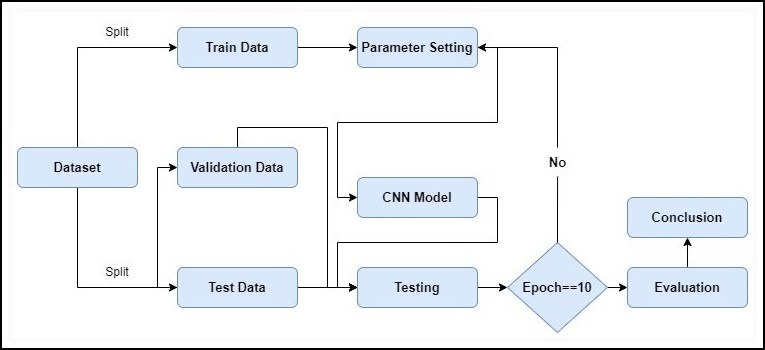
\includegraphics[width=8.8cm, height=4cm]{Tomato Final Flowchart.jpg}
\caption{Flowchart of the proposed work}
\label{fig: Figure 1}
\end{figure}

\subsection{Data Pre-Processing}
There is not a major need for extra effort to normalise the photos because the PlantVillage dataset already contains pre-processed images with little to no distortion.\\
Along with the initial dataset, data augmentation techniques including rotation, flipping, and zooming were used on the training set to increase the dataset size and improve the CNN model's robustness.\\
Overall, the dataset for classifying tomato leaf illnesses employed in this effort is extensive, varied, and representative of many tomato diseases.



% \subsection{Temporal Attention module}
% Inspired by the various attention techniques~\cite{.....}, we employ a temporal attention module to capture temporal dependencies among snippets. After that, the attention scores are multiplied with the feature vectors to detect anomaly events. Thus, the temporal attention module allows the network to concentrate on the more important snippets.


\subsection{CNN - Convolutional Neural Network}

CNNs are a specific type of neural network designed specifically for processing visual input like images and video. By using many layers, CNNs have demonstrated astounding efficacy in a variety of image and video processing tasks. The model's convolutional layers employ learnable filters to glean important information from the input pictures. The computational complexity is then decreased by downsampling these collected characteristics using pooling layers. In order to enable accurate classification, fully linked layers are then used to map the retrieved characteristics to the relevant output classes. With its use in object identification, semantic segmentation, and picture classification, CNNs have transformed computer vision. The focus of recent research has been on using CNNs to automatically identify and classify plant diseases, particularly those that harm tomato leaves. Popular deep learning architectures like AlexNet and GoogleNet were tested to diagnose tomato leaf disease; customised variants of the ResNet architecture proved to be the most accurate.\\

The deep neural network structure ResNet50, which was first introduced in a study by Zhang et al. \cite{Zhang_2021_WACV} in 2015, was used in the machine learning model that we used. 

ResNet's basic idea is to use residual connections, which let information travel over numerous stacked levels to facilitate a smooth flow through the network. This is achieved by including skip connections, which create a shortcut between layers by adding the input of one layer to the output of another.

ResNet was able to circumvent the issue of disappearing gradients that frequently bedevils deep neural networks by including these skip connections. Very deep networks can be trained more effectively because the skip connections make it simpler for gradients to flow backward through the network during backpropagation.

ResNet is available in several variations, with ResNet50 being a well-liked version that employs 50 layers. In the realm of visual computing, the ResNet50 architecture has won considerable acclaim for its outstanding performance, particularly in tasks like scene segmentation, object tracking, and image recognition. It has raised the bar and established new standards in these areas.

\section{Experiment}
\subsection{Dataset}
The study used the 54,000 labelled photos from 14 distinct crop types in the publicly available PlantVillage dataset, which is available to anybody. A total of 20,639 tomato leaf photos, each measuring 256 by 256 pixels, were included in this collection. These pictures of tomato leaves were divided into ten different categories, with one category depicting healthy leaves and nine indicating various sick situations. The dataset was split into three subsets to prepare it for analysis: the training set, which includes the remaining 70\% of the photographs, the test set, which includes another 15\% of the images, and the validation set, which includes 15\% of the images. The RGB colour space was used to represent each image in the collection, which was stored in the JPEG format as shown in the Figure~\ref{fig: Figure 2} .

 \begin{figure}[H]
 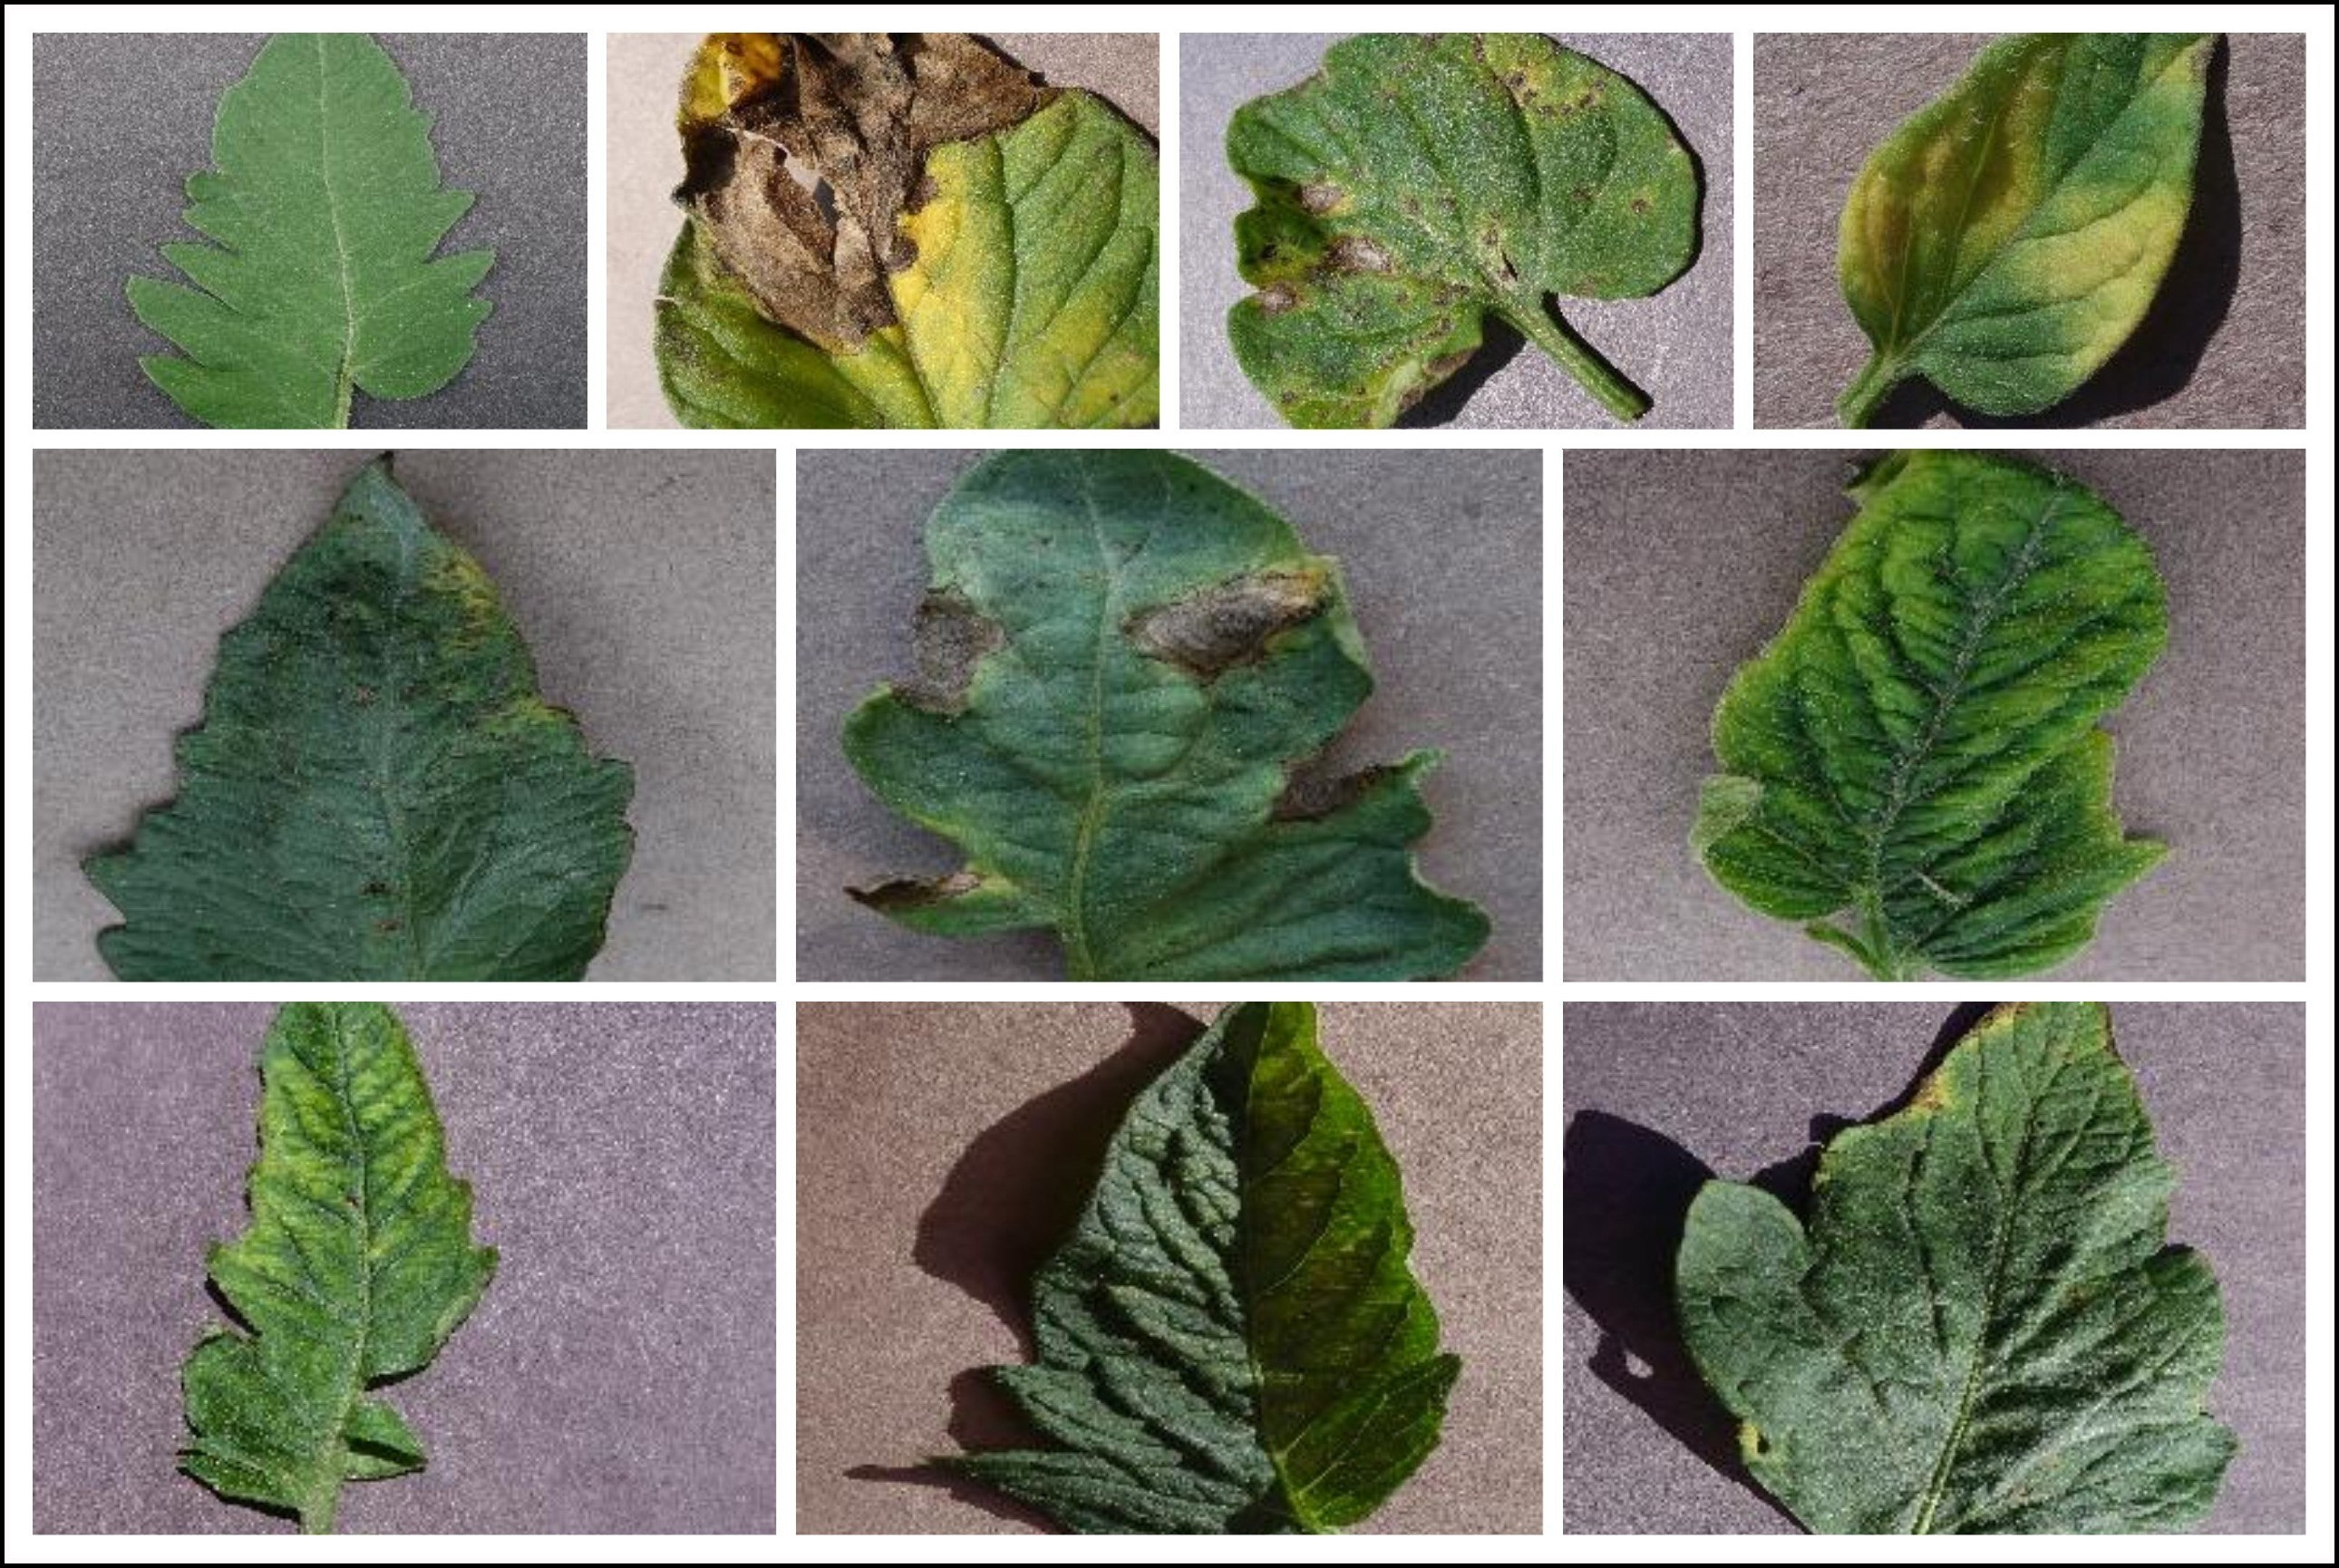
\includegraphics[width=8.8cm, height=5cm]{Tomato Dataset.jpg}
\caption{Images from the datasets used}
\label{fig: Figure 2}
\end{figure}
 
\subsection{Evaluation Measure}
The suggested CNN model's efficiency for categorising tomato leaf diseases was evaluated using a variety of assessment indicators. Classification accuracy was the primary assessment parameter employed. This statistic determines the percentage of test set pictures that were correctly classified in comparison to all images.
\\ 


Along with accuracy, the efficacy of the suggested model is assessed using a variety of metrics, including recall, precision, and F1-score. Precision evaluates the link between accurately predicted positive cases and all projected positive instances, whereas recall quantifies the association between effectively anticipated positive occurrences and all true positive instances. The F1-score, a comprehensive statistic, is used to compute the harmonic mean of accuracy and recall.\
In general, a combination of these assessment measures may be used to assess how effectively the proposed CNN model distinguishes between tomato leaf diseases and to compare it to other current models.




\subsection{Experiment setting} 
Using the Python programming language and a number of libraries, including TensorFlow, Keras, and OpenCV, the suggested CNN model for identifying tomato leaf disease is put into practise. On a computer system with an i7-6800 3.4 GHz CPU, a 2 GB NVIDIA Geforce GPU, and 16 GB RAM, the model is run. With a learning rate of 0.001 and a batch size of 256, the Adaptive Moment Estimation optimizer is used to train the model over the course of 10 epochs. Three separate sets, with relative proportions of 70\%, 15\%, and 15\%, were created from the collection of tomato leaf images: a training set, a validation set, and a testing set.


\section{Results and Discussion}
% In this section, we present and discuss the experimental results obtained 

The model's performance was assessed using the F1-score, recall, accuracy metrics, and precision in addition to the confusion matrix. The training accuracy was claimed to be 97.8\%, whereas the maximum validation accuracy attained was 95.6\%. The deep learning model for classification was found to be successful with an average validation accuracy of 95\%.

 \begin{figure}[H]
 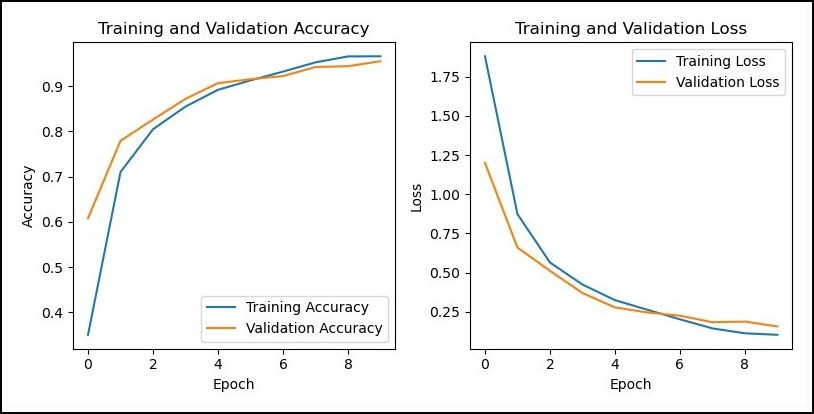
\includegraphics[width=8.9cm, height=4.5cm]{Tomato Accuracy and Loss.jpg}
\caption{The model's accuracy  and loss was assessed during both the training and validation stages.}
\label{fig: Figure 3}
\end{figure}

The graphs show the model's accuracy and loss in a visual manner. As demonstrated in Figure~\ref{fig: Figure 3}, the accuracy graph exhibited a continuous increase in accuracy before stabilising, while the loss graph showed a steady decline in loss before doing the same. These graphs provide us an understanding of how well the model performs and show that it is a useful tool for classifying the 10 various types of tomato leaf diseases. By providing a clear visualization of the model's progress, these graphs enhance our understanding of its capabilities and reinforce its value as a reliable tool for disease classification.

 \begin{figure}[H]
 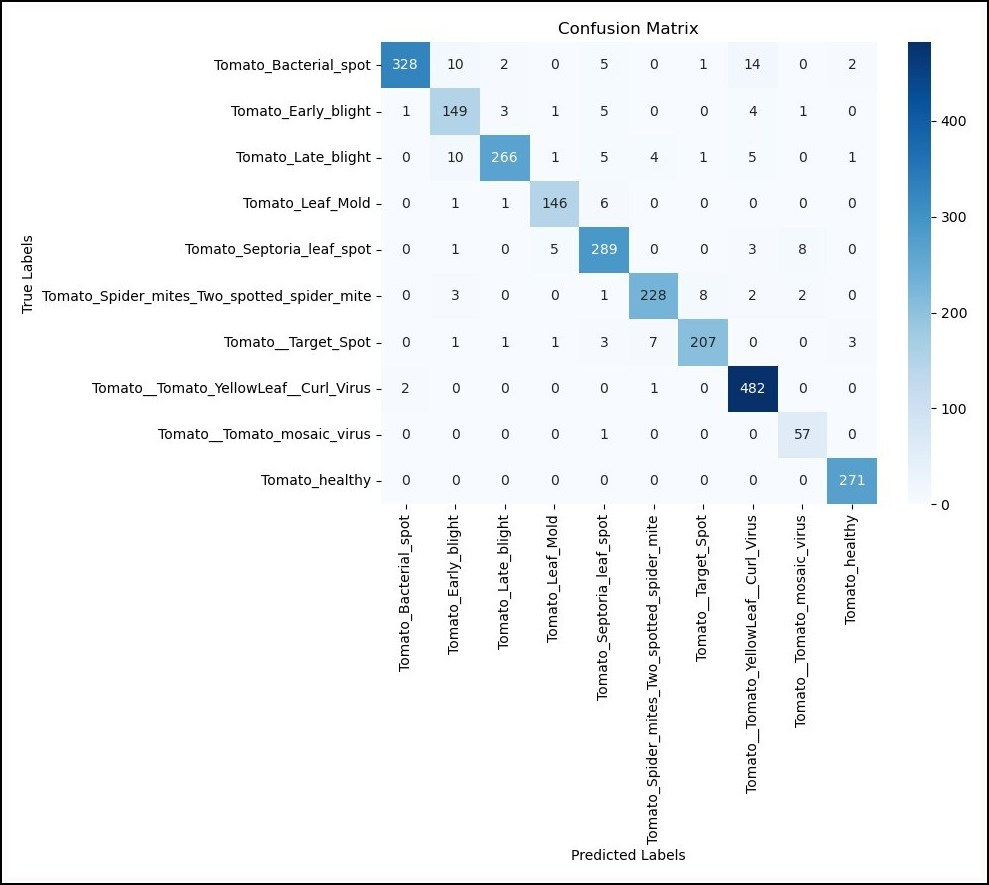
\includegraphics[width=8.8cm, height=5cm]{Tomato Confusion Matrix.jpg}
\caption{Confusion matrix for the model used in the paper}
\label{fig: Figure 4}
\end{figure}

 \begin{figure}[H]
 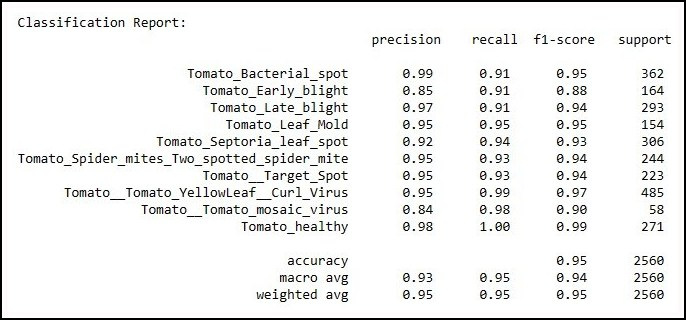
\includegraphics[width=8.8cm, height=4cm]{Tomato Stats.jpg}
\caption{Accuracy, Precision, Recall and F1-Score for the used model}
\label{fig: Figure 5}
\end{figure}

We conducted a comprehensive evaluation of image classification models using the confusion matrix and performance metrics including accuracy, precision, recall, and F1 score. The confusion matrix allowed us to visually analyze the model's performance by comparing the predicted labels with the ground truth labels. From the confusion matrix, we derived the accuracy, which measures the overall correctness of the classification. Additionally, precision provided insights into the model's ability to correctly identify positive instances, recall evaluated its capability to capture all positive instances, and the F1 score considered the balance between precision and recall as shown in the figure~\ref{fig: Figure 4} and figure~\ref{fig: Figure 5}.
  
\section{Conclusion and Future Work}
In India, a considerable section of the population is supported by the agricultural industry, and crop disease detection is crucial to the sector's development and sustainability. There are a number of ways available for spotting illnesses in tomato plants, each with their own benefits and drawbacks. The Plant Village dataset is used in this study to suggest a simple method for classifying and identifying tomato leaf diseases using a convolutional neural network (CNN) model. The programme can provide exact predictions by examining patterns and characteristics in leaf photos. Data augmentation techniques are used to increase the system's performance and robustness. The suggested approach has a noteworthy accuracy rate of 92-95\% while using little processing power. The performance of the model could be improved in future study by examining other optimizers, learning rates, and newer architectures. Further advancements might potentially be achieved by optimising the training settings to shorten training times. The approach is adaptable for disease detection in other plants, such as apples, potatoes, cucumbers, and brinjal, extending its use beyond tomatoes.

% \section*{Acknowledgment}
% This work is supported by the FIST project of Department of Science and Technology, Govt. of India. We thank Mr. xxxxxxxxxxxxxxxxxx for his assistance with language editing, and proofreading. 
%\section{References}
\bibliographystyle{IEEEtran}
\bibliography{santos_bib}

\end{document}







